%!TEX root = talk612.tex

%!TEX root = thesis.tex

\documentclass[a4paper]{article}
\usepackage{amsthm}
\usepackage[utf8]{inputenc}
\usepackage{csquotes}
\usepackage[english]{babel}
\usepackage{graphicx}
\usepackage{enumitem}
\usepackage{subcaption}  %ALLOWS SUBFIGURES
\usepackage{wrapfig}

\usepackage[draft]{fixme}
\fxsetup{theme = color}
\definecolor{fxnote}{rgb}{0.0000, 0.6000,0.0000}
\definecolor{fxwarning}{rgb}{1.0000,0.5490,0.0000}
\definecolor{fxerror}{rgb}{1.0000,0.2706,0.0000}
\definecolor{fxfatal}{rgb}{1.0000,0.0000,0.0000}
\usepackage[backend=biber, giveninits =true, isbn=false, url=false, maxbibnames=100]{biblatex}
\usepackage{hyperref}

%Theorems
\newtheorem{thrm}{Theorem}
\newtheorem{lemma}[thrm]{Lemma}
\newtheorem{prop}[thrm]{Proposition}
\newtheorem{remark}[thrm]{Remark}

\theoremstyle{definition}
\newtheorem*{defi}{Definition}

%%BeginIpePreamble
\usepackage{amsmath}
\usepackage{amssymb}
\usepackage{amsopn}

\newcommand{\scr}[1]{\mathcal{#1}}
\newcommand{\Z}{\mathbb{Z}}
\newcommand{\F}{\mathbb{F}}
\newcommand{\R}{\mathbb{R}}
\newcommand{\N}{\mathbb{N}}
\newcommand{\Q}{\mathbb{Q}}


%Operators
\newcommand{\id}{\operatorname{Id}}



%braces etc
\newcommand{\braces}[1]{\left\lbrace {#1} \right\rbrace}
\newcommand{\sqbr}[1]{\left\lbrack {#1} \right\rbrack }
\newcommand{\abs}[1]{\left\lvert {#1} \right\rvert }
\newcommand{\ceil}[1]{\left\lceil{ #1 } \right\rceil}
\newcommand{\floor}[1]{\left \lfloor {#1}\right\rfloor}
\newcommand{\parens}[1]{\left( {#1} \right)}


%utility
\newcommand{\inv}[1]{{#1}^{-1}}
\newcommand{\half}{\frac{1}{2}}
\newcommand{\third}{\frac{1}{3}}
\newcommand{\goes}{\rightarrow}
\newcommand{\nin}{\not \in}
\newcommand{\sm}[1]{\setminus \braces{#1} }

%vectors and matrices
\newcommand{\zerov}{\vec{0}}
\newcommand{\onev}{\vec{1}}

\newcommand{\twovec}[2]{\parens{ \begin{array}{c}#1 \\ #2\end{array} }}
\newcommand{\threevec}[3]{\prens{ \begin{array}{c}#1 \\ #2\\#3 \end{array} }}
\newcommand{\fourvec}[4]{\parens{ \begin{arr\newcommand{\ifftext}{if and only if }ay}{c}#1 \\ #2\\#3\\#4 \end{array} }}
\newcommand{\twomatrix}[4]{\parens{\begin{array}{cc}#1 & #2 \\ #3 & #4 \end{array}  }}
\newcommand{\twodiagmatrix}[2]{\parens{\begin{array}{cc}#1 & 0 \\ 0 & #2 \end{array}  }}

%%%%THIS THESIS
\newcommand{\intplus}{\operatorname{Int^{+}}}
\newcommand{\interior}{\operatorname{Int}}
\newcommand{\spl}{\operatorname{split}}
\newcommand{\mrg}{\operatorname{merge}}


\newcommand{\ext}[1]{\bar{#1}}
\newcommand{\tightext}[1]{\bar{#1}_t}
\newcommand{\dualgraph}[1]{\G(#1)}
\newcommand{\extdualgraph}[1]{\G_{\scr E}(#1)}



\newcommand{\W}{\scr W}
\renewcommand{\P}{\scr P}
\newcommand{\C}{\scr C}
\newcommand\restrict[1]{\raisebox{-.5ex}{$|$}_{#1}}
\newcommand{\restC}[1]{\ensuremath{\C\restrict{#1}}}

%p is for pole
\newcommand{\pN}{\mathrm{N}}
\newcommand{\pS}{\mathrm{S}}
\newcommand{\pE}{\mathrm{E}}
\newcommand{\pW}{\mathrm{W}}

\newcommand{\cpath}{\C \setminus \braces{\pS}} %cycle path

\newcommand{\rel}{\text{regular edge labeling }}

%%EndIpePreamble


%bib stuff
\bibstyle{plain}

\addbibresource{../thesis.bib}


\title{Investigations}
\author{Sander Beekhuis}
\date{\today} %\today%


\begin{document}
\maketitle



A \emph{valid} extended graph (or valid EG) is a extended graph containing no seperating $4$ cycles.



\section{Cornerassignments without separating $4$-cycle are not necessarily one-sided}
  False, consider the isocahedron minus one edge as EG. This is the only valid corner assignment of the underlying graph since otherwise there will be an interior vertex of degree 4.
  \begin{figure}[h]
    \centering
    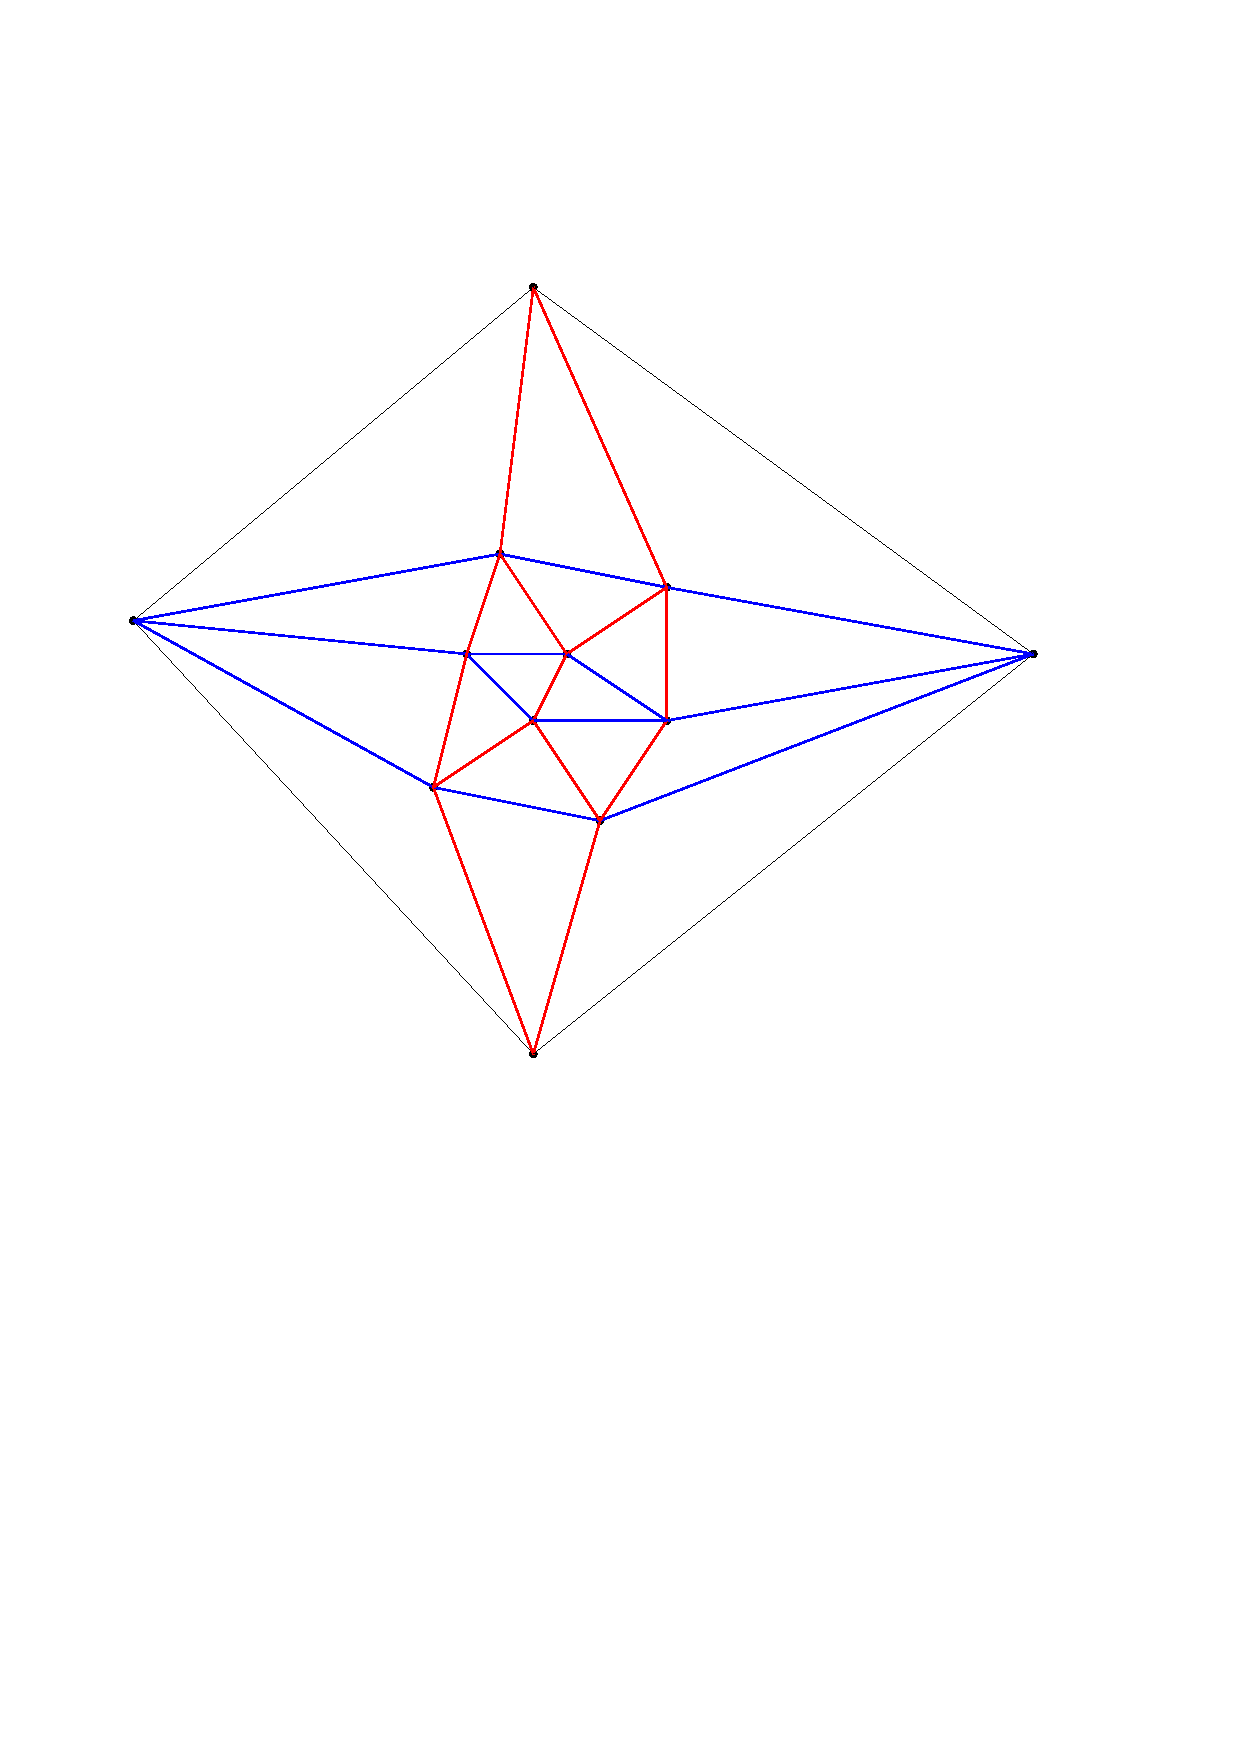
\includegraphics[scale=.5]{img/isoc_m1_colored}
    \caption{A coloring of the isocahedron minus one edge}
    \label{fig:}
  \end{figure}

  Then it also follows that there is no one-sided colorings of this graph.


\section{A link with triangulations}

  There is a close link between valid EG's and 5-connected triangulation's via the \emph{point-completion} of the EG. Unfortuantly this is not $5$ connected due to the completing point.


  One can also try the \emph{edge-completion}. This unfortunatly also doesn't work

  The dual of a $5$-connected traingulation is a cyclically $5$-connected cubic graph.

  It might very well be that the dual of the point-completion is a strongly cyclically $4$-connected graph. We know how to make these graphs due to [Barnnete 1973].

  We can probably do this while maintaining a dual REL. This algorithm is actually really close to Kant and He's edge contraction. However it seems hard to maintain any quality in this solution.
  \fxnote{Show with figure}

  While we do this we probably also don't destroy flips. So that would mean that every valid EG leads to a graph that's at best $(2, \infty)$.


  \begin{con}
    All valid extended graphs can be generated from a base graph and a set of moves. Similarly to 5 connected triangulations.
  \end{con}


  \subsection{When we remove an edge from a 5-connected triangulation we get a valid extended graph without any separating 4-cycle.}

  \begin{proof}
    Let $G$ be any 5 connected plane triangulation. By Lemma \ref{lm:5connIsNoSep4C} we know that $G$ has no separating $4$-cycle. If we consider any edge $e$ and $\tilde{G} = G \setminus{e}$ then certainly $\tilde{G}$ also has no separating $4$-cycle. Since any separating $4$-cycle of $\tilde{G}$ would have already been one of $G$.
  \end{proof}

  Note that a $5$-conneted graph minus one edge is not necessarily again $5$-connected.

  Unfortunately not all extended graphs without separating $4$-cyles can be generated this way. Conside for example the graph in Figure \ref{fig:ure}. This example has been checked by hand and python on not containing 4cycles.

  \begin{figure}[h]
    \centering
    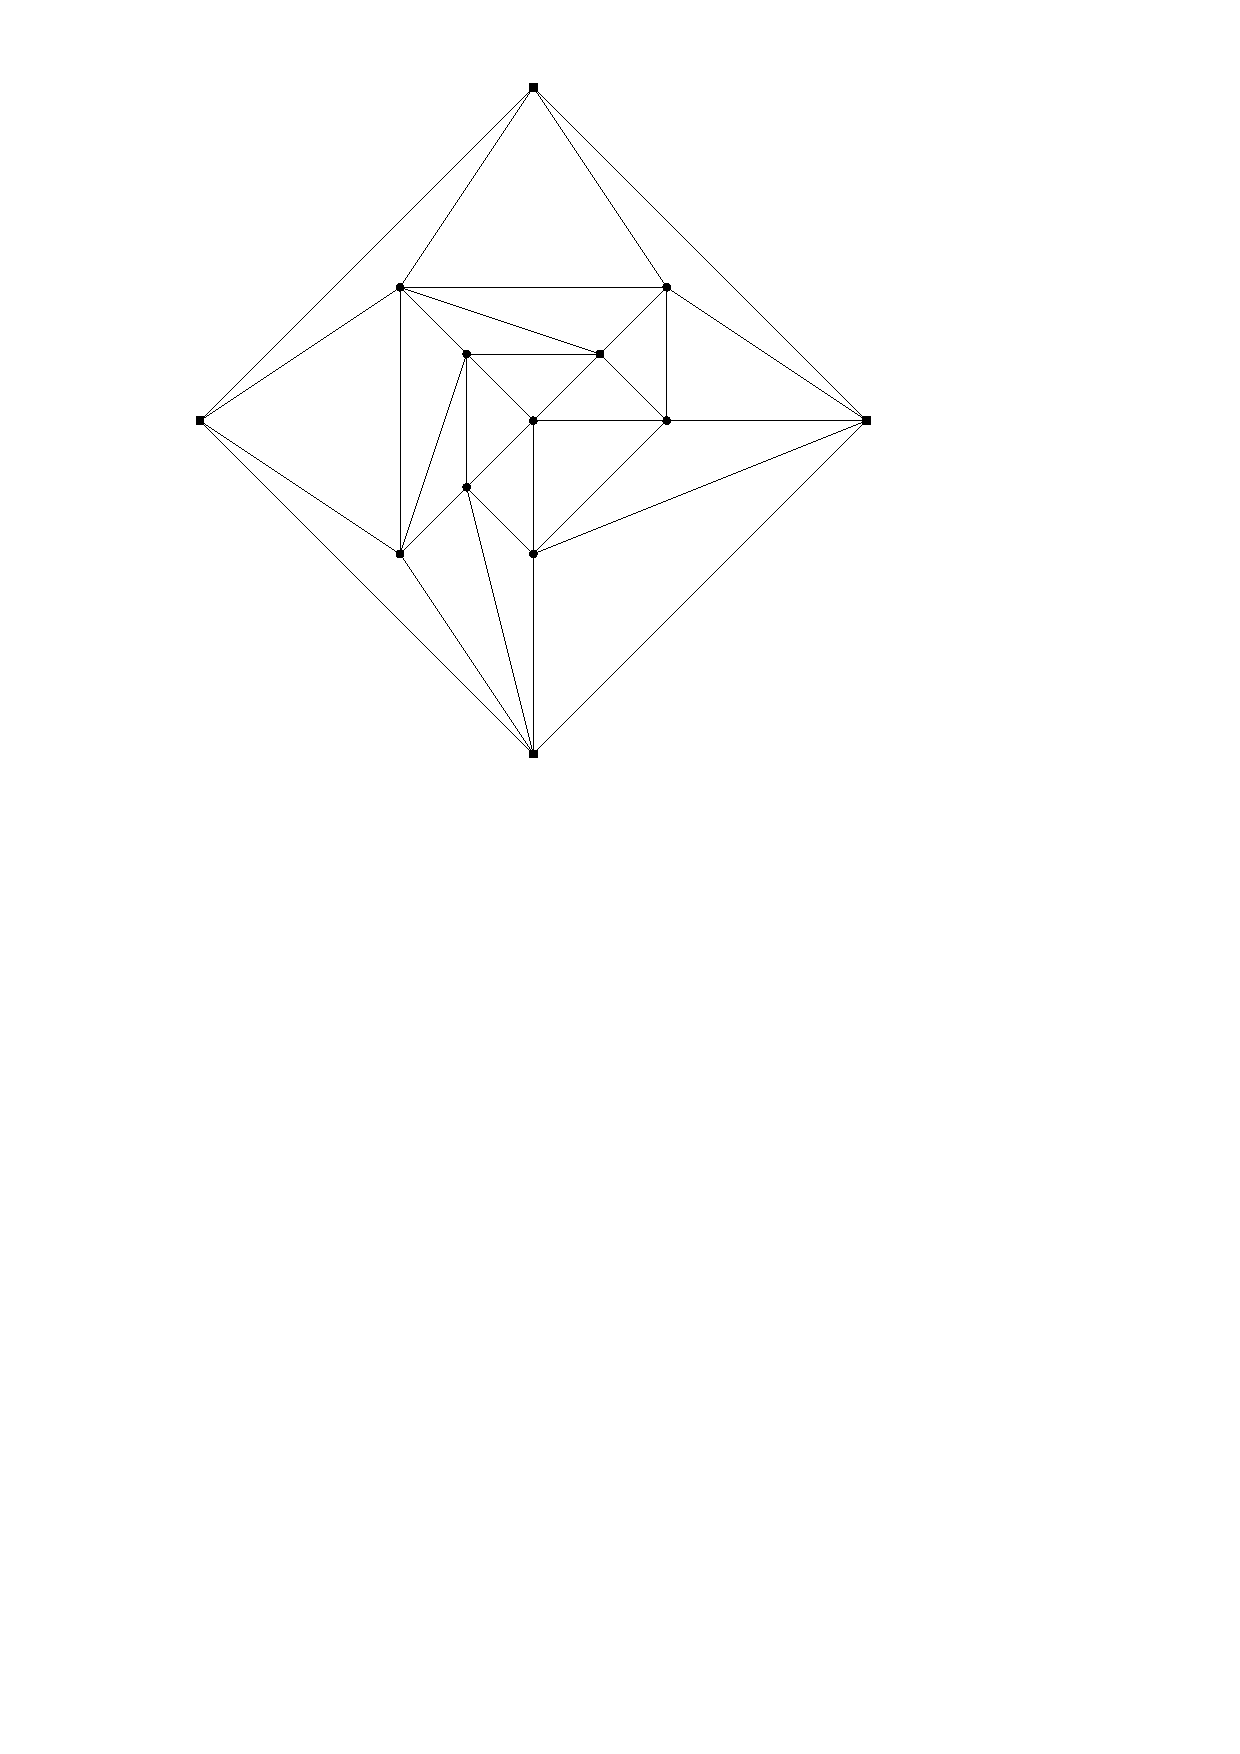
\includegraphics[scale=1]{NoSeperating4CycleButAdddingEdgeBackInIsBad.pdf}
    \caption{}
    \label{fig:ure}
  \end{figure}


  \subsection{The dual of a REL}
  We can look at the dual problem of finding a REL. This is natural when we are doing steps as described above.


  In this setting the interior vertex requirements become

  Every cycle is colored with a nonzero number of red, blue, red and blue patches while for every vertex holds that not all adjacent edges can be of the same color.




\section{Failed attempts}
\paragraph{Planar separoatrs}
I tried something using planar separators. Unfortunately both sides seem to depend to much upon each other. I.e. we can't properly separate using a boundary. It might be fruitful to see the interior as separating.


\paragraph{Building a REL}
We can build a REL using the steps of constructing a 5-connected triangulation. Unfortunatly it is a bad one.
Base graph and lots of step 3.

\section{The current state of the algoritmh}



\subsection{A new way to deal with chords, diagonally}
A figure says more then a thousand words: so see Figure \ref{fig:removechordOld} and \ref{fig:removeChordNew}

\begin{figure}[h]
  \centering
  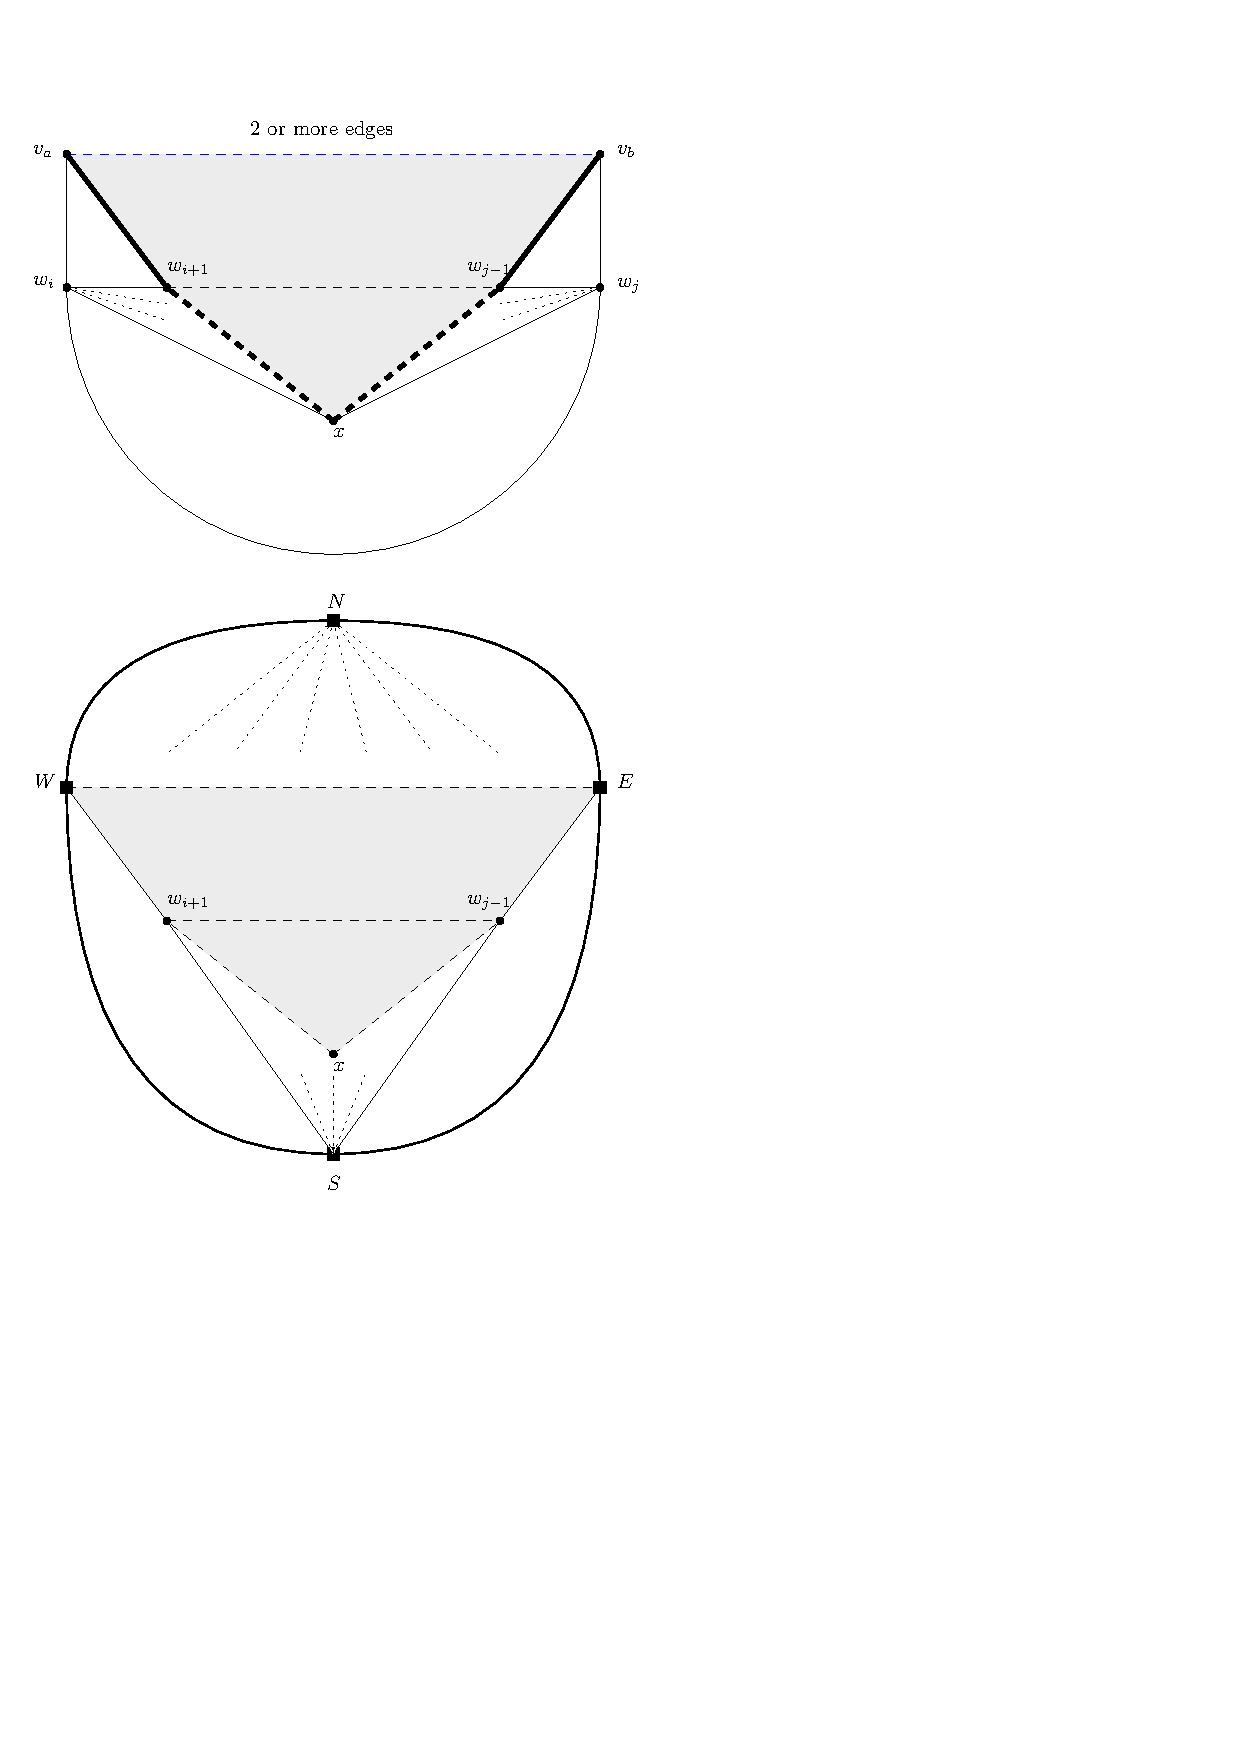
\includegraphics[scale=.6]{img/removeChordOld.pdf}
  \caption{Removing a chord, the old way}
  \label{fig:removechordOld}
\end{figure}

The old way could lead to a $4$-cycle containing the new $N$ vertex or $S$ vertex. The new way only has this problem with the $N$ vertex.

But if this is the case we know how the fence above the chord looks so we can solve our problems.

\begin{figure}[h]
  \centering
  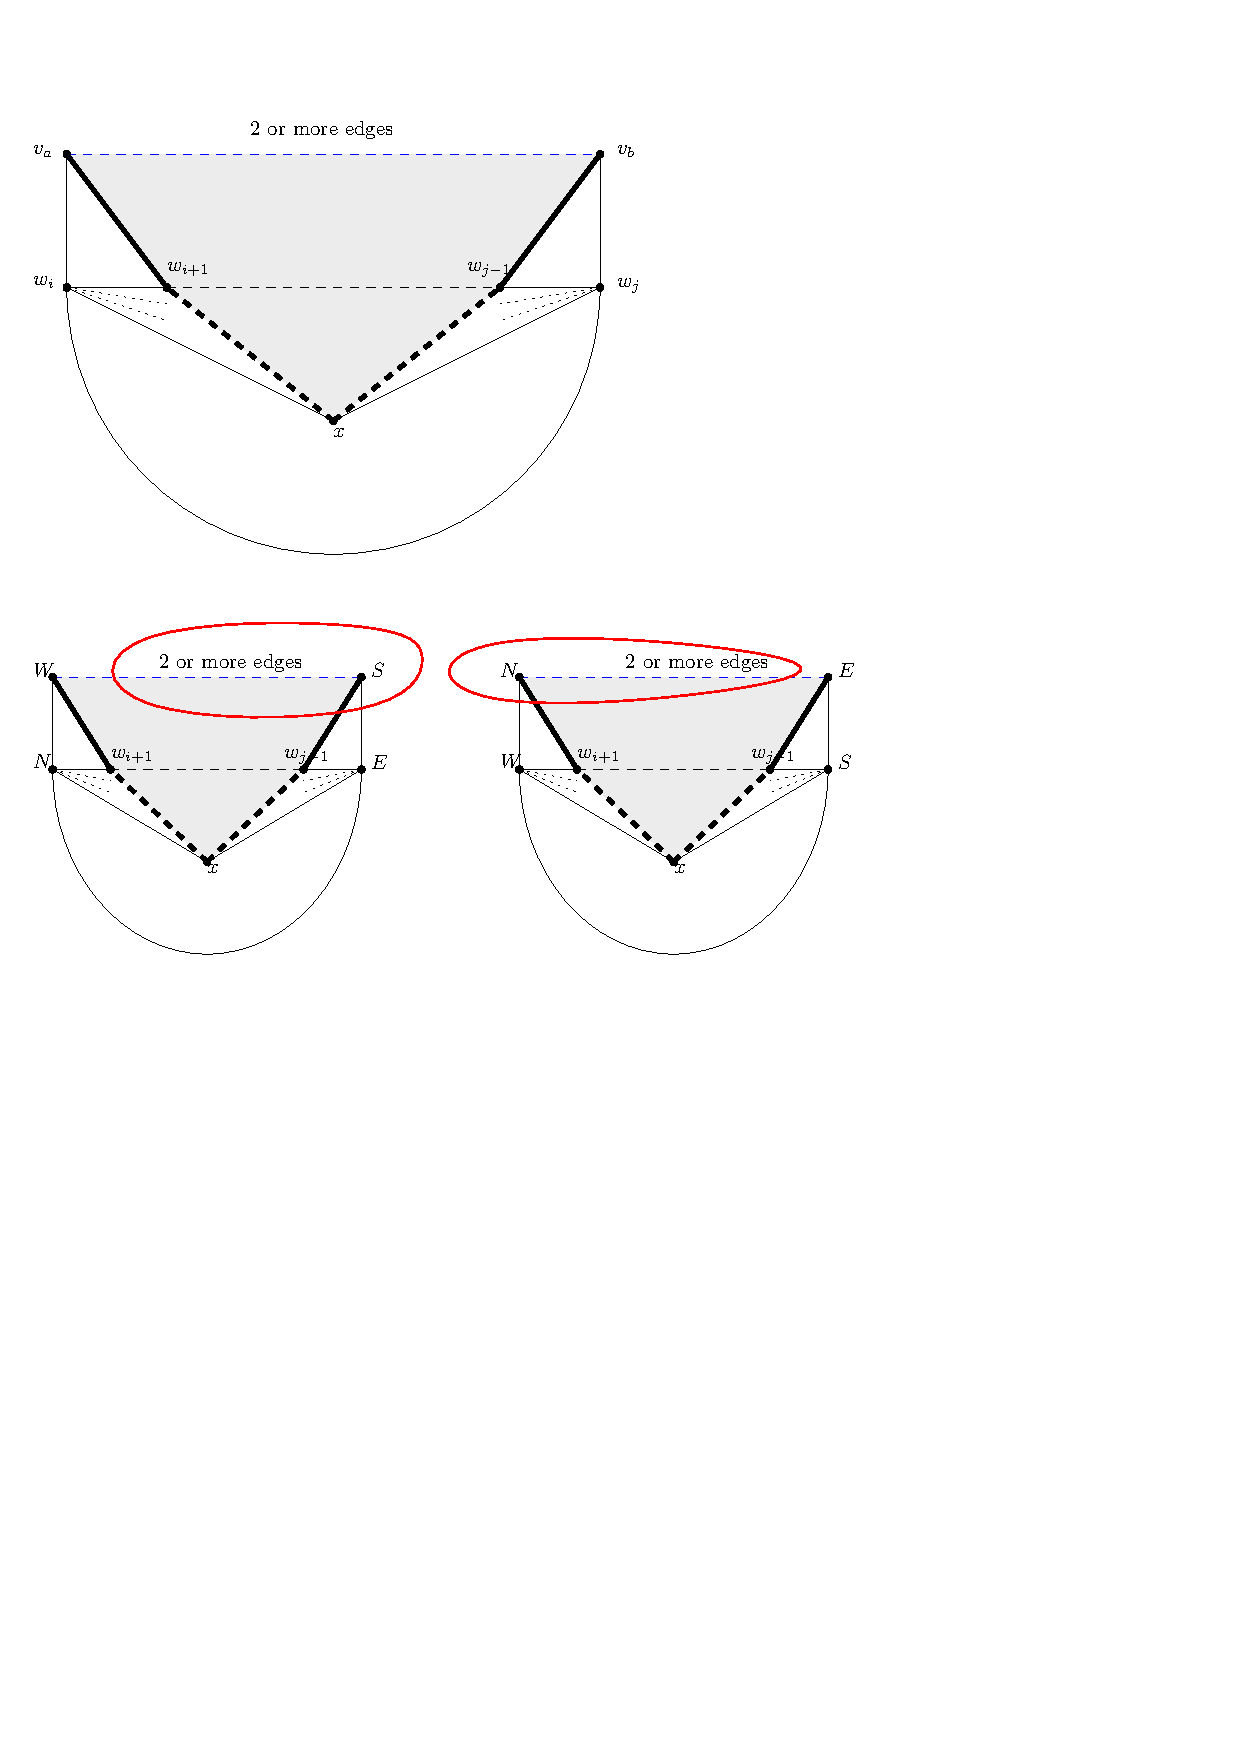
\includegraphics[scale=.6]{img/removeChordNew.pdf}
  \caption{Removing a chord, the new way}
  \label{fig:removeChordNew}
\end{figure}


\subsection{A new way to deal with Non-simple points, evading them.}

Note that a non-simple point is not something that has to occur. It is something that exists due to an unfortunate sequence of fences.


\subsection{Algorithm Plan}

\begin{enumerate}
  \item We find fences taking care that we don't hit any NSP while also not doing something horrible for red. \emph{Not quite sure about the exact implementaion}
  \item We scan bottom-up for chords and mustflip edges. We orient chords such that:
  \begin{enumerate}
    \item A chord above another chord is oriented such that it has a \emph{preventable Z}
    \item A chord above a must flip does not form a $Z$
    \item Two mustflips above each other are prevented by doing some \emph{moves}
  \end{enumerate}

  \item We flip some non-offending edges in the remaining large blue faces. Which we can hopefully do due to some edge load invariant we have maintained.
\end{enumerate}


\section{Open research quenstions}
  \begin{enumerate}
    \item Can one always complete a correct partial collering? (Advancing per vertex)
    \item is the degree $4$ vertex at the north pole of the cord graph really a problem. Why? What should we do about it?
    \item How do paths inside a cycle behave? Why do we have the $4$-cycle property
  \end{enumerate}

\section{TODO}
  \begin{enumerate}
    \item   Completly read Barnnete1973. Maybe any onderstanding of this paper will advance a dual REL approach.
  \end{enumerate}



\section{Misc results}
  \begin{lemma}
    \label{lm:5connIsNoSep4C}
    For plane triangulations having no separating 4-cycle is the same as being 5-connected
  \end{lemma}

  \begin{proof}
  We will show this by contraposition (i.e. having a separating 4-cycle is equivalent to not being 5-conencted).
  If a triangulation $G$ has a separating 4-cyle then the nodes of this $4$-cycle are a $4$-cutset and $G$ is not $5$-connected.
  On the other hand, if a triangulation is not $5$ connected there is a cutset $X$ of size at most $4$. Removing $X$ splits $G$ into several connected components. By the property that $G$ maximally planar the nodes in $X$ must form a cycle. (They should form a closed curve preventing edges from the one component to the other one.)
  \end{proof}


  \paragraph{Cubic graph with only faces of degree 5}
  Is unique

  \paragraph{Why do we actually care about chords?}
  Beacuse we otherwise get pockets of untreated nodes

  \begin{con}
    This problem might be FTP in high degree nodes or NP-hard
  \end{con}
    I don't actually think it's true. But I did spend some time looking for an obvious reduction


    \subsection{Other ideas}
    Maybe we can uses Birkenhoff and find sets that are flipped a certain number of times

    Some combined red/blue step

    A planar separator going trough faces of a low degree (can be large, but this are relatively harmless faces if an edge flip goes trough them).

    Inside the separator we must have no crossing paths. (This might be restrictive on colorings inf the inside is just a path.)

    Planar separator on primal?


    Build a REL using consttuction steps. If it goes wrong, reverse change color and try again.

    Can we always finish a valid partial coloring? (Of dual and or primal)


    Induction on construction steps?
    %\listoffixmes

    There is some structure to the interior of cycles. Can we understand this structure?

    The current approach is to try and draw graphs that don't work

\printbibliography
\end{document}
